\documentclass{iopjournal}
% NOTE: references.bib is in biblatex format. To switch to \bibliographystyle{iopart-num}
% (native iopjournal), convert bib entries: journaltitle->journal, date->year.
% For now, biblatex is used for compatibility with the existing .bib file.
\usepackage{lmodern}
\usepackage{float}
\usepackage{siunitx}
\usepackage{booktabs}
\usepackage{subcaption}
\usepackage{graphicx}
\graphicspath{
  {./images/}
  {./images/Mushroom/}
  {./images/Bronze/}
  {./images/Nb3Sn/}
  {./images/intro/}
  {./images/intro/Nb3SnProperties/}
  {./images/Metallurgy/}
}
\usepackage[
    backend=biber,
    sorting=none,
    doi=false,
    url=false
]{biblatex}
\addbibresource{references.bib}

\begin{document}

\articletype{Paper}

\title{RF Performance of Nb$_3$Sn Films on Bronze Substrates Formed by the Hot-Bronze Route}

\author{Andre Robert Juliao$^{1*}$ and Lance D Cooley$^{1}$}

\affil{$^1$Applied Superconductivity Center, National High Magnetic Field Laboratory,
Florida State University, Tallahassee, FL 32310, USA}

\affil{$^*$Author to whom any correspondence should be addressed.}

\email{arj14c@fsu.edu}

\keywords{Nb$_3$Sn, thin films, hot-bronze, superconducting radio frequency, surface resistance, quality factor}

\begin{abstract}
Nb$_3$Sn thin films were deposited on Cu-15\,wt.\%\,Sn bronze substrates using a hot-bronze sputtering route in which Nb was sputtered onto a heated (\qty{715}{\degreeCelsius}) bronze surface, causing immediate formation of Nb$_3$Sn. A post-reaction variant subjected the hot-bronze films to an additional \qty{715}{\degreeCelsius} anneal. Two-inch disk samples were characterized by critical temperature ($T_c$) measurements and by quality factor ($Q$) measurements in a mushroom cavity at SLAC National Accelerator Laboratory. The hot-bronze samples achieved $Q = 1.2\times10^6$, while the hot-bronze plus post-reaction samples achieved $Q = 5.5\times10^5$, both measured against a Cu host cavity at zero applied magnetic field. The reduction in $Q$ after post-reaction is attributed to grain growth in the underlying bronze substrate, which roughens the Nb$_3$Sn surface. These results provide the first RF validation of Nb$_3$Sn films fabricated via the Cu-Sn ternary bronze route and establish the hot-bronze method as a viable path toward high-quality Nb$_3$Sn coatings on copper-compatible substrates.
\end{abstract}


\section{Introduction}

Superconducting radio-frequency (SRF) cavities achieve quality factors many orders of magnitude higher than normal-conducting alternatives, enabling energy-efficient particle accelerators and sensitive quantum-sensing instruments. Bulk Nb cavities, the present standard, are fundamentally limited to accelerating gradients below \qty{50}{MV/m} and cannot sustain superconductivity above \qty{9.2}{\kelvin} or in fields exceeding \qty{0.4}{\tesla}~\cite{padamseeRFSuperconductivity2009}. Nb$_3$Sn offers a compelling upgrade path: with $T_c = \qty{18.3}{\kelvin}$ and an upper critical field $H_{c2} \approx \qty{30}{\tesla}$, it theoretically doubles the achievable accelerating gradient and remains superconducting in fields relevant to dark-matter axion haloscopes (\qty{9}{\tesla}) and high-field magnet applications~\cite{gurevichUseNotUse2011, posenMeasurementHighQuality2022}.

The dominant fabrication route for Nb$_3$Sn SRF cavities reacts bulk Nb cavities with Sn vapor near \qty{1100}{\degreeCelsius}, achieving $Q_0 \sim 10^{10}$--$10^{11}$ at zero field~\cite{Posen:2018zjb}. This process is incompatible with copper substrates, which soften and recrystallize above \qty{700}{\degreeCelsius}~\cite{okudaFabricationTestingLband1991}. Cu is attractive as a cavity substrate because of its high thermal conductivity and established manufacturing base, motivating the development of low-temperature Nb$_3$Sn routes. Adding Cu to the Nb-Sn reaction reduces the required temperature to \qty{650}--\qty{750}{\degreeCelsius} via the ternary Cu-Nb-Sn reaction pathway~\cite{suenagaChemicalCompositionsGrain1983}. This pseudo-binary bronze route has been exploited for decades in Nb$_3$Sn wire manufacturing~\cite{ambrosioNb3SnHighField2015} and is now being adapted for thin-film cavity fabrication~\cite{luDevelopmentPerformanceFirst2022, withanageRapidNbSn2021}.

The hot-bronze method, introduced in~\cite{withanageRapidNbSn2021} for thin-film applications, deposits Nb via magnetron sputtering directly onto a Cu-Sn bronze substrate held at $\sim$\qty{715}{\degreeCelsius}. Arriving Nb atoms immediately react with Sn at the bronze surface, forming Nb$_3$Sn in situ. This contrasts with the conventional post-reaction approach, in which Nb is deposited cold and then annealed separately. The hot-bronze method produces a fine-grained columnar Nb$_3$Sn microstructure (Zone-2 Thornton morphology) and critical temperatures of \qty{14}--\qty{15}{\kelvin} on $\alpha$-bronze substrates, limited primarily by compressive strain from the coefficient of thermal expansion (CTE) mismatch upon cooldown~\cite{ekinStrainScalingLaw1980, withanageRapidNbSn2021}.

Critical temperature measurements indicate film quality but do not directly assess RF surface resistance. Quality factor measurements in a resonator are the decisive test for SRF applications. This work reports the first RF characterization of hot-bronze Nb$_3$Sn films, performed at SLAC National Accelerator Laboratory using a mushroom cavity test structure~\cite{tantawiSuperconductingMaterialsTesting2007}. Two-inch bronze-substrate samples --- one hot-bronze and one hot-bronze plus post-reaction --- were tested at zero applied field. Results are discussed in the context of microstructure and inform the development of Cu-compatible SRF coatings.


\section{Experimental detail}

\subsection{Substrate preparation and Nb$_3$Sn synthesis}

Cu-15\,wt.\%\,Sn ($\alpha$-bronze, 9\,at.\%\,Sn) substrates were used as both the mechanical substrate and the Sn reservoir. Two-inch diameter, \qty{3}{\milli\meter} thick disks were mechanically polished to a mirror finish using progressive SiC paper (400--1200 grit), diamond slurry (5--\qty{1}{\micro\meter}), and vibratory colloidal silica (\qty{0.05}{\micro\meter}). Substrates were ultrasonically cleaned in acetone and isopropyl alcohol, dried with compressed air, and loaded into a UHV magnetron sputtering chamber (base pressure \qty{e-9}{\torr}).

Two processing routes were employed, both using Nb deposited from a 2-inch magnetron gun at \qty{250}{\watt} with \qty{8}{\milli\torr} Ar working gas. Pre-sputtering behind a closed shutter for 3 minutes removed surface contaminants from the target prior to deposition.

\begin{itemize}
    \item \textbf{Hot-bronze}: The bronze substrate was pre-heated to $\sim$\qty{715}{\degreeCelsius} and held at this temperature throughout Nb deposition. Arriving Nb atoms reacted immediately with Sn at the bronze surface, forming Nb$_3$Sn in situ during deposition~\cite{withanageRapidNbSn2021}.

    \item \textbf{Hot-bronze + post-reaction}: Following the hot-bronze deposition above, the sample was held at \qty{715}{\degreeCelsius} for an additional 3 hours in the same UHV chamber. The residual Sn in the bronze continued to feed the growing Nb$_3$Sn layer, increasing stoichiometric uniformity.
\end{itemize}

Target Nb$_3$Sn thickness was $\sim$\qty{1}{\micro\meter} in both cases.

\subsection{Critical temperature characterization}

The critical temperature onset $T_c$ was measured by recording magnetic moment ($m$) vs.\ temperature using a SQUID magnetometer (Quantum Design MPMS-5). Samples were zero-field cooled to $\sim$\qty{4}{\kelvin}, after which a \qty{1}{\milli\tesla} field was applied parallel to the film surface and data were collected in \qty{0.1}{\kelvin} increments up to \qty{20}{\kelvin}. $T_c$ onset is defined as the highest temperature at which the normalized moment deviates from zero; the transition width $\Delta T_c$ spans 90\%--10\% of the transition.

\subsection{Mushroom cavity RF measurement}

Quality factor measurements were performed at SLAC National Accelerator Laboratory using a mushroom cavity~\cite{tantawiSuperconductingMaterialsTesting2007, thomsonSRF2015Whistler2015}. The mushroom cavity consists of a 2-inch flat disk sample clamped against a host cavity (Cu in this case), with RF surface currents concentrated radially across the sample face. Higher-order modes localize the currents to small regions of the cavity, reducing sensitivity to boundary effects at the sample edge. Thermometers on the back of the sample monitored temperature; cooling was provided by a cold head attached to the cavity. The quality factor was extracted from $S_{21}$ transmission measurements as a function of temperature from \qty{4}{\kelvin} to room temperature.

The Cu host cavity introduces a systematic limitation: because Cu at 4~K has surface resistance $R_s \sim \qty{10}{\milli\ohm}$, the host cavity's contribution to the total loss is not negligible. A superconducting Nb host cavity would reduce this error and better isolate the sample contribution. The current results therefore represent a lower bound on the intrinsic sample $Q$.


\section{Results}

\subsection{Critical temperature}

The superconducting transition curves for the bronze coupon samples (representative of the 2-inch disks sent to SLAC) are shown in Fig.~\ref{fig:WenuraBronzeTc}. The hot-bronze sample (H2) exhibits $T_c \approx \qty{14}{\kelvin}$, while the hot-bronze + post-reaction sample (PR2) exhibits a slightly higher $T_c$ with a broader transition. Both samples show $T_c$ below the maximum of \qty{18.3}{\kelvin}, consistent with compressive strain imposed by CTE mismatch between Nb$_3$Sn and the bronze substrate upon cooldown~\cite{ekinStrainScalingLaw1980, withanageRapidNbSn2021}.

\begin{figure}[htb]
    \centering
    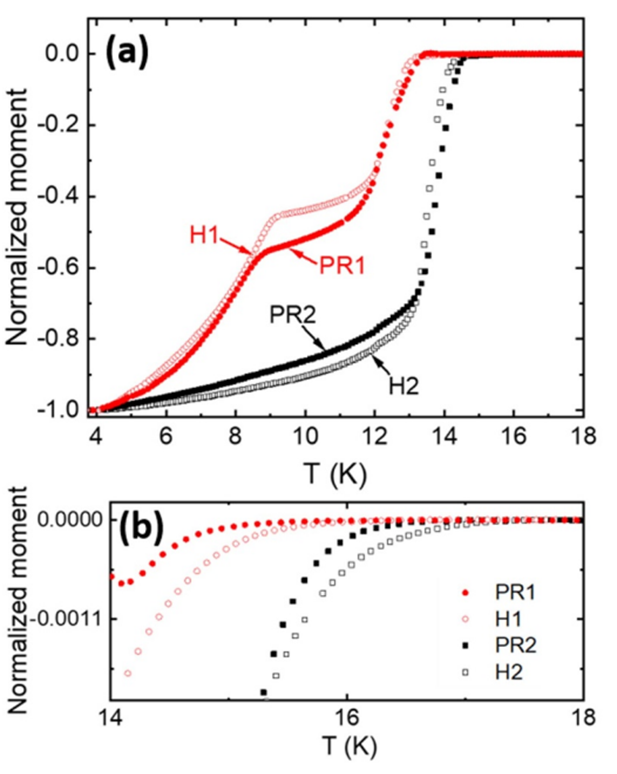
\includegraphics[width=0.55\linewidth]{images/Mushroom/WenuraBronzeTc.png}
    \caption{Critical temperature curves for the bronze coupon samples representative of those sent to SLAC. H2: hot-bronze; PR2: hot-bronze + post-reaction~\cite{withanageRapidNbSn2021}.}
    \label{fig:WenuraBronzeTc}
\end{figure}

\subsection{Sample morphology}

The 2-inch disk samples after synthesis are shown in Fig.~\ref{fig:2inchBronzeSub}. Both disks display a rolling texture inherited from the bronze substrate. The post-reaction sample exhibits a darker region in the lower left, indicating a microstructurally distinct area, possibly from non-uniform grain growth in the bronze during the extended anneal.

\begin{figure}[htb]
    \centering
    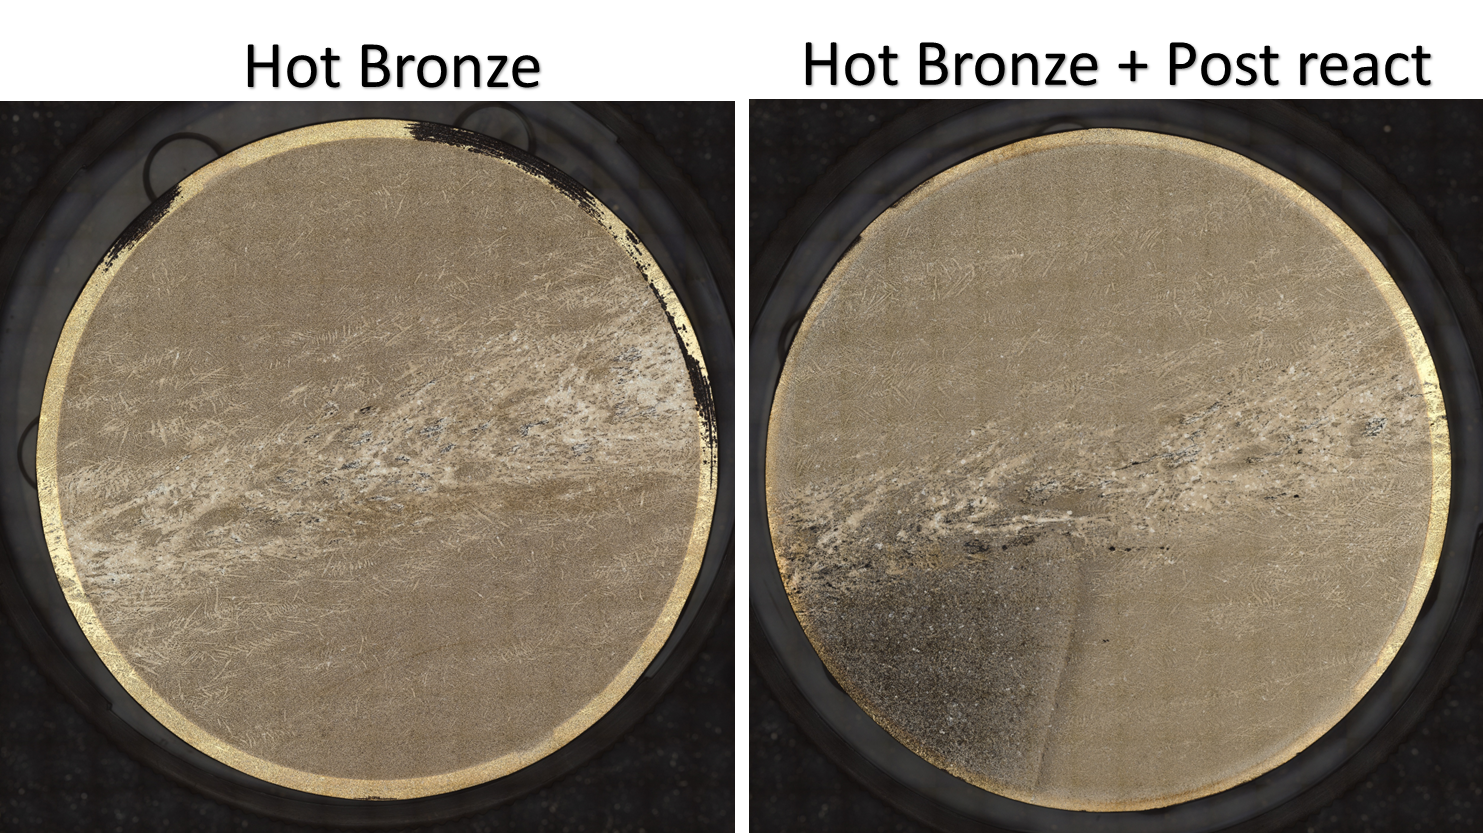
\includegraphics[width=0.85\linewidth]{images/Mushroom/2inchBronzeSub.png}
    \caption{Two-inch bronze substrate disks after Nb deposition and reaction. Left: hot-bronze sample. Right: hot-bronze + post-reaction sample. Rolling texture from the bronze substrate is visible in both. The darker region in the post-reaction sample (lower left) indicates locally distinct microstructure.}
    \label{fig:2inchBronzeSub}
\end{figure}

\subsection{Quality factor vs temperature}

The quality factor measured in the SLAC mushroom cavity is shown in Fig.~\ref{fig:MushroomQvsT}. The hot-bronze sample achieved $Q = 1.2 \times 10^6$ and the hot-bronze + post-reaction sample achieved $Q = 5.5 \times 10^5$ at base temperature (\qty{4}{\kelvin}). Both Nb$_3$Sn samples demonstrate substantially higher $Q$ than a bare Cu reference sample, confirming superconducting contributions from the film. The shaded regions indicate measurement uncertainty arising from the Cu host cavity.

\begin{figure}[htb]
    \centering
    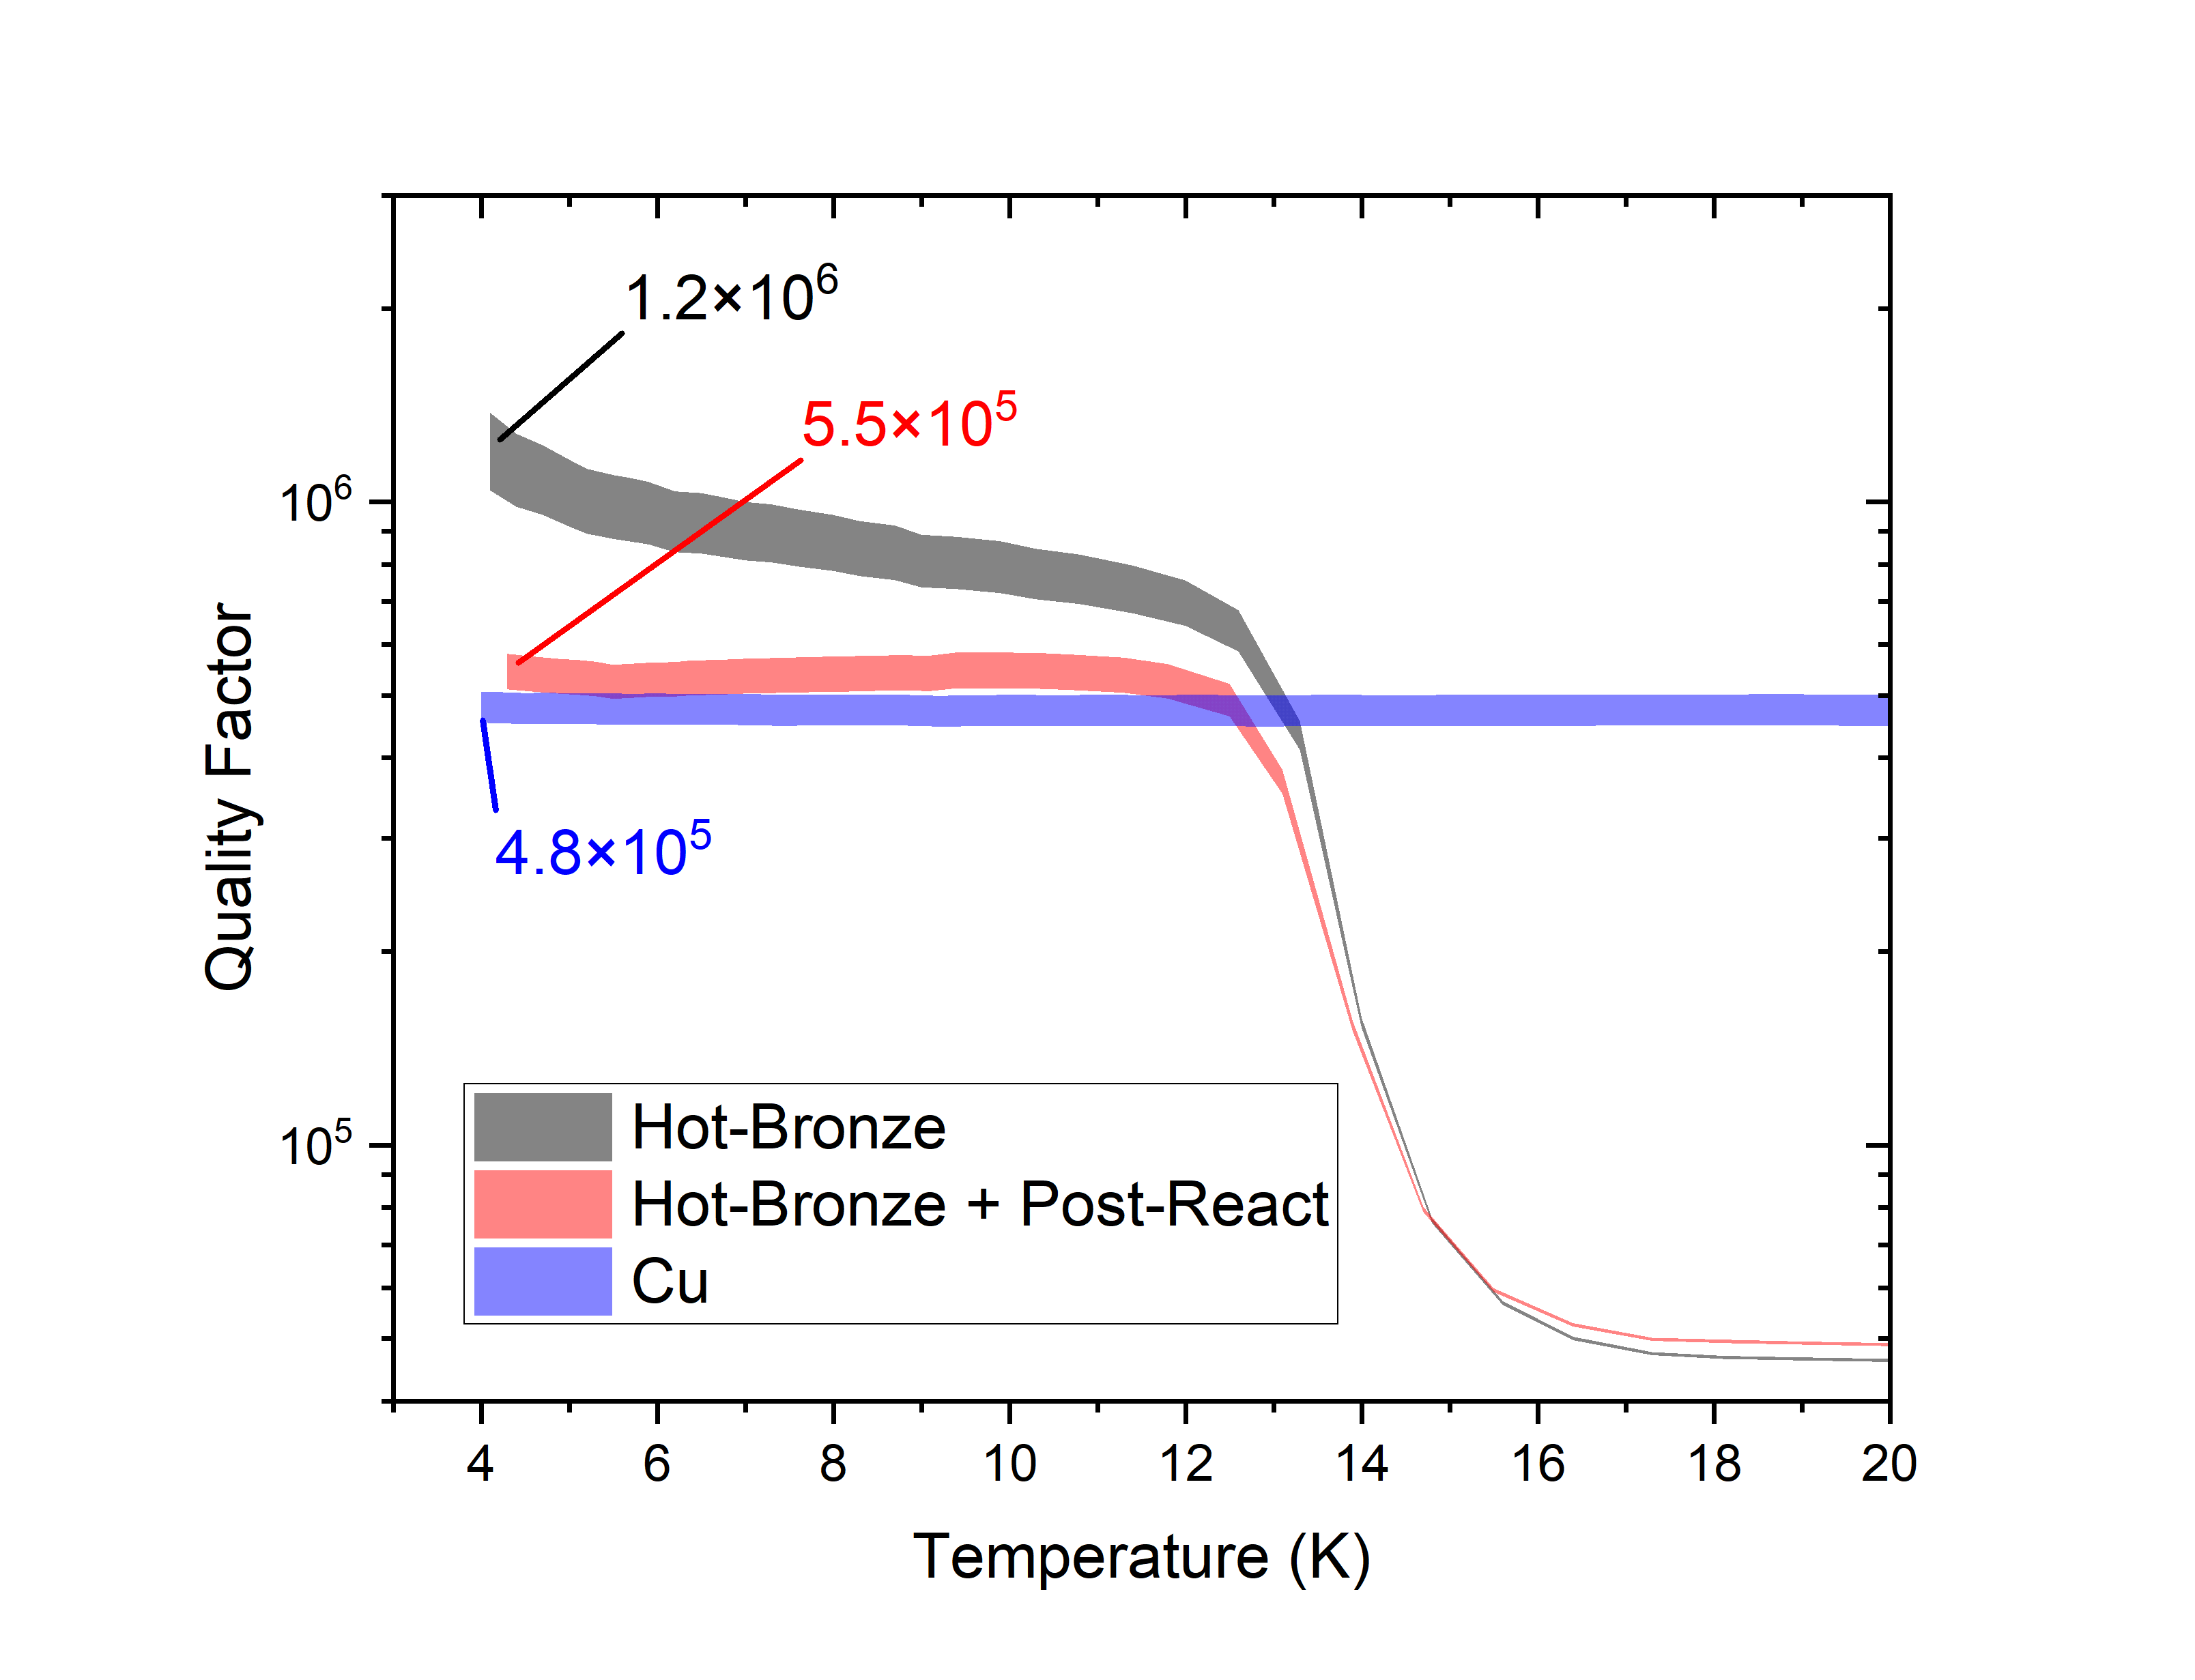
\includegraphics[width=0.7\linewidth]{images/Mushroom/QvsTMushroomCavityNew.png}
    \caption{Quality factor vs temperature measured in the SLAC mushroom cavity for the hot-bronze (filled) and hot-bronze + post-reaction (open) 2-inch bronze samples. Shaded regions indicate measurement uncertainty from the Cu host cavity contribution. Both Nb$_3$Sn samples exceed the bare Cu reference.}
    \label{fig:MushroomQvsT}
\end{figure}


\section{Discussion}

The hot-bronze sample achieves higher $Q$ than the post-reaction sample despite $T_c$ curves suggesting the post-reaction sample has marginally higher Sn content. This counterintuitive result is attributed to microstructural differences in the bronze substrate. The extended post-reaction anneal at \qty{715}{\degreeCelsius} drives grain growth in the $\alpha$-bronze, roughening the substrate and consequently the Nb$_3$Sn film surface. Elevated surface roughness increases residual resistance through enhanced magnetic flux trapping and vortex pinning at surface irregularities~\cite{leeGrainboundaryStructureSegregation2020}. The patterning visible at the center of both disks (Fig.~\ref{fig:2inchBronzeSub}) is a rolling artifact and is consistent with earlier observations in~\cite{withanageRapidNbSn2021}; this texture is present in both samples and is not the source of the $Q$ difference.

The TEM microstructure of a hot-bronze film on bronze (Fig.~\ref{fig:TEMHotBronze}) reveals Cu segregated at some grain boundaries. In accelerator applications, grain boundary impurities increase residual resistance~\cite{leeGrainboundaryStructureSegregation2020}; the same mechanism likely contributes to the residual surface resistance observed here. High-temperature annealing (\qty{1100}{\degreeCelsius}) has been shown to reduce grain boundary Sn and improve $Q$ in Sn-vapor-processed cavities, but this is not compatible with Cu substrates.

\begin{figure}[htb]
    \centering
    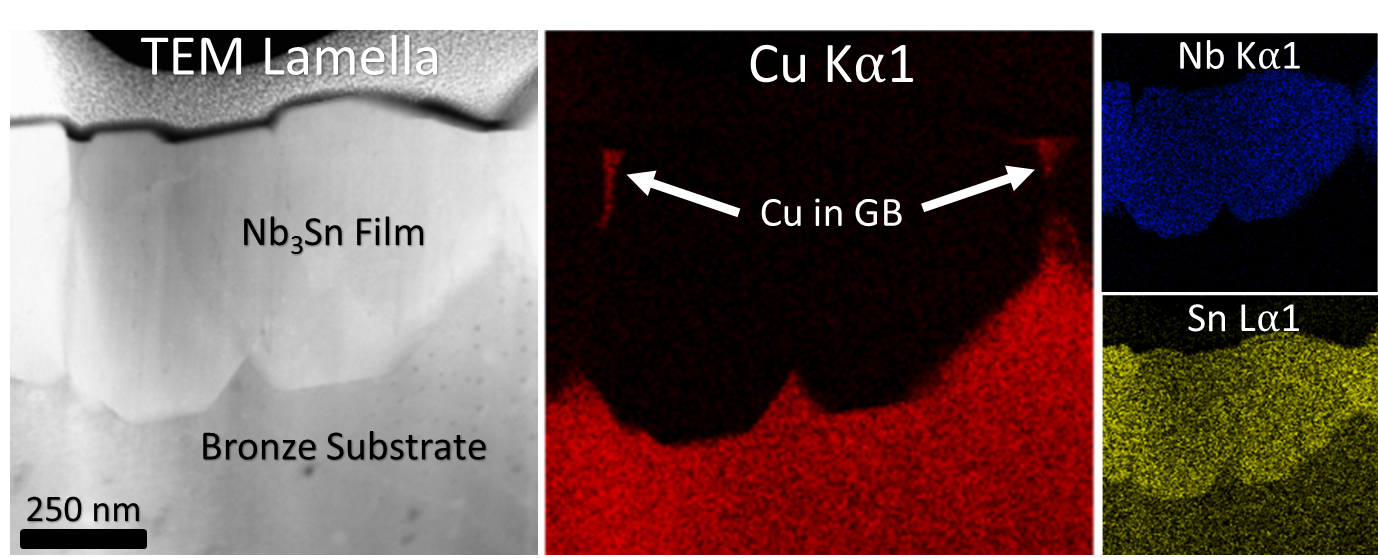
\includegraphics[width=0.85\linewidth]{images/Bronze/TEMHotBronze.png}
    \caption{TEM image of a hot-bronze Nb$_3$Sn film on a bronze substrate, showing Cu segregated at some grain boundaries.}
    \label{fig:TEMHotBronze}
\end{figure}

The Cu host cavity introduces substantial uncertainty in the absolute $Q$ values: the Cu surface resistance at 4~K ($R_s \sim \qty{10}{\milli\ohm}$) is comparable to the Nb$_3$Sn contribution, making the extracted sample $Q$ sensitive to the precise Cu cavity geometry and surface condition. A Nb host cavity, planned by SLAC for follow-on measurements, would reduce this error by an order of magnitude. The current values of $Q \sim 10^6$ should therefore be regarded as lower bounds on the intrinsic film quality.

These results validate the hot-bronze route as an RF-capable path to Nb$_3$Sn films on Cu-compatible substrates. The measured $Q = 1.2 \times 10^6$ is comparable to first-generation Nb-on-Cu coatings for SRF applications, and represents a starting point for further optimization. Reducing grain boundary impurities, improving substrate surface preparation, and transitioning to Cu substrates with diffusion barriers are the primary levers for improvement.


\section{Conclusions}

Hot-bronze and hot-bronze + post-reaction Nb$_3$Sn films deposited on Cu-15\,wt.\%\,Sn bronze substrates were characterized for RF surface resistance using the SLAC mushroom cavity. The hot-bronze method achieved $Q = 1.2 \times 10^6$, outperforming the hot-bronze + post-reaction sample ($Q = 5.5 \times 10^5$), despite the post-reaction sample showing marginally higher $T_c$. The $Q$ degradation after post-reaction is attributed to bronze grain growth during the extended anneal, which roughens the Nb$_3$Sn surface and increases residual resistance. These results provide the first RF measurement of Nb$_3$Sn films formed by the Cu-Sn ternary bronze route, establishing the hot-bronze method as a viable fabrication path. The \qty{715}{\degreeCelsius} processing temperature is compatible with copper substrates, making this approach extensible to fully Cu-based SRF cavities and axion dark-matter haloscopes operating in multi-tesla fields.

\ack
The authors thank the SLAC National Accelerator Laboratory for mushroom cavity access. Work at the Applied Superconductivity Center was supported by [funding source TBD].

\section*{Data availability statement}
Data supporting this study are available from the corresponding author upon reasonable request.

\printbibliography

\end{document}
